\documentclass[main.tex]{subfiles}
\begin{document}


\chapter{Concept} \label{chap:Concept}


\begin{figure}[H]
    \centering
    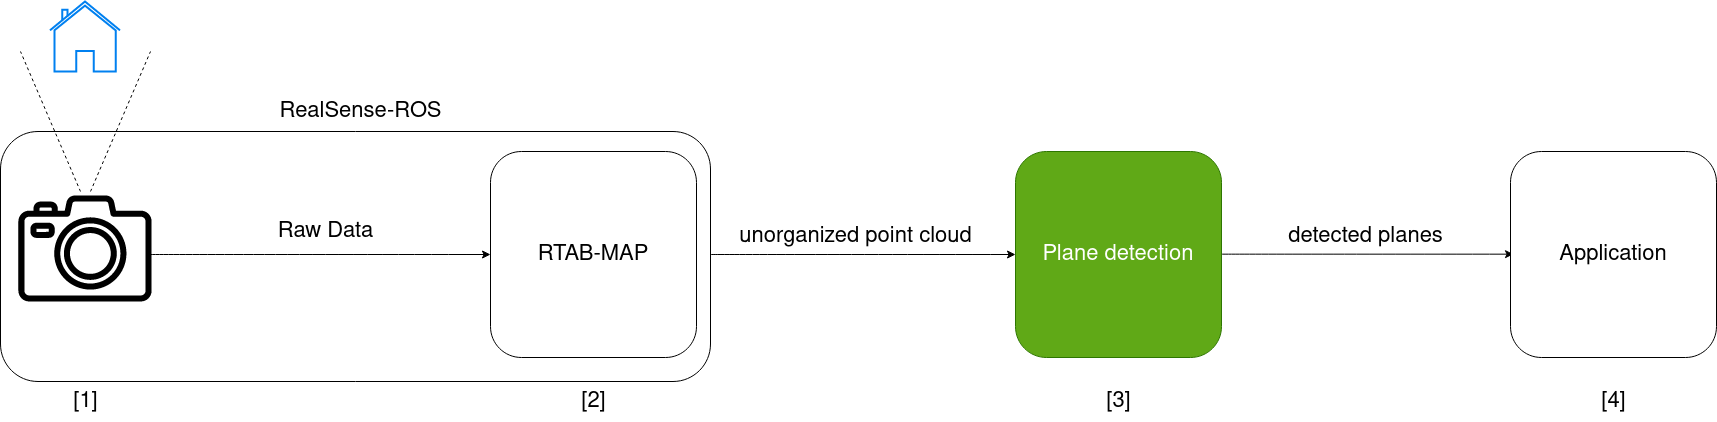
\includegraphics[width=15 cm]{images/concept_specific.png}
    \caption[Concrete Concept Graphic]{The procedure of the plane detection process. The specialized sensor records data ([1]), which is passed to
        a SLAM algorithm ([2]). After map assembly, a point cloud is handed to a plane detection algorithm ([3]).
        The detected planes are given to a use-case-specific application ([4]).}
    \label{fig:concept}
\end{figure}

Many AR and VR Systems integrate plane detection into their software, some use it only to calculate the ground floor while others use plane detection to
build a smaller model of the environment.
Figure~\ref{fig:concept} shows a generic block diagram of such a VR/AR system including plane detection.
In general, the environment is continuously recorded by a specialized sensor which is usually a camera([1]). A SLAM algorithm then integrates the new data into its already existing map([2]). The map, in form of a point cloud,
is subsequently passed to a plane detection algorithm([3]). The algorithm performs the necessary steps to detect all planes inside the current map and passes the planes to the application([4]).
The application would then further process those planes, e.g., by creating a live visualization of them or by assisting the movement of visually impaired people~\cite{Carranza_Estrella_Zaidi_Carranza_2021}.

To remove any noticeable lag in the application, the plane detection step has to run under a temporal restriction, henceforth referred to as \textit{real-time}.
We state a more precise definition in Section~\ref{sec:realtime}.

When creating such a AR/VR system, the choice of plane detection algorithm is naturally of great importance. The problem is that most published algorithms are not inherently comparable.
Often different datasets or metrics are used, which precludes comparison by quantification. Alternatively, algorithms are not comparable by internal functionality
because many methods require different inputs, and the format of the planes differs accordingly. All in all, selecting a single 'best' algorithm is impossible solely based on the metrics presented in their
respective work.

To answer the question of which algorithm is best and whether it is real-time capable, we make a unified comparison of plane detection algorithms.
To perform this evaluation, we need the following:

\begin{enumerate}
    \item \label{enum:pda}Appropriate plane detection algorithms,
    \item \label{enum:ds} a useful dataset \textit{and}
    \item \label{enum:rt} a definition of \textit{real-time}.
\end{enumerate}
The following sections are dedicated to them.


% Roter Faden:
% \begin{itemize}
%     \item generic view on AR + VR system
%     \item Describe the building blocks in there
%     \item Point out that the decision on the "best" PDA is not clear
%     \item Tell me why that is not clear!
%     \item Get me going on those PDA
%           \begin{itemize}
%               \item describe my view on the world
%               \item show marco that table
%               \item describe what these values mean and why they are important
%           \end{itemize}
% \end{itemize}

\section{Selection of Plane Detection Algorithms}\label{sec:pdaselection}
% SECTION get me going on those PDA 
% FIXME describe my view on the world
% FIXME show marco that table
% FIXME describe what these values mean and why they are important
%!SECTION - 

Since most algorithms differ in certain aspects, it is not possible to compare them all uniformly. Furthermore, not all algorithms have the same motivation and therefore focus on different things.
For example, evaluating an algorithm in a scenario it has not been designed for would not yield meaningful results.
It is, therefore, necessary to first define objective criteria to superficially determine which algorithm seems to be relevant for the context of this work.


\subsection{Criteria}
In the following paragraphs, we define and outline appropriate criteria for the objective assessment of plane detection algorithms.

\paragraph{Type of Input}\label{par:input}
The first criterion is the type of input expected by a plane detection algorithm.
Allowing vastly different input types is likely to render the evaluation more complicated, if not impossible because an equivalent transformation
between two input types is not always possible. 
Usually, the data representation of the recorded environment falls into one of three categories:
% FIXME wahrscheinlich eher in den BG
% \begin{table}[H]
%     \centering
%     \begin{tabular}{c|c|c}
%         \textbf{Input Types}             & \textbf{Value Types} & \textbf{Memory Layout} \\ \hline
%         \textbf{Organized Point Cloud}   & 3D Coordinates       & 2D Matrix              \\
%         \textbf{Unorganized Point Cloud} & 3D Coordinates       & 1D Array               \\
%         \textbf{Depth Image}             & Distances to Sensor  & 2D Matrix              \\
%         \textbf{RBG Image}               & RGB                  & 2D Matrix
%     \end{tabular}
%     \caption{Possible inputs for plane detection algorithms.}
%     \label{tab:inputs}
% \end{table}
\begin{itemize}
    \item \textit{unorganized} or \textit{unstructured point cloud} (UPC)
    \item \textit{organized} or \textit{structured point cloud} (OPC)
    \item \textit{(depth-) image} (D-/I)
\end{itemize}
% FIXME in den Background verschieben ,hier nur kurz den unterschied umreissen 

OPC and UPC both describe point clouds in the cartesian coordinate system. The primary difference is that the 3D coordinates inside
an organized point cloud are saved in a 2D grid, while the unorganized cloud resembles an unsorted 1D array.
Like OPC, depth images are a 2D grid of values. However, in contrast to the 3D coordinates of an OPC, the data points of depth images
are the distances to the sensor.



\paragraph{Detected Plane Format} \label{subsec:planeformat}
Which specific representation the detected planes take the form of is also essential.
If no uniform output type can be determined, consequently, no uniform metric for comparison can also be found.


Often the found planes are saved as a list of 3D points, henceforth referred to as inliers, which were assigned to a plane.
Another often-plane output format is the cartesian equation of a plane described by a normal vector $n$ and a vector $d$.

In methods that work on image data, found planes are often described by an image mask or pixels that belong together.

Finally, some methods use plane detection as a means to an end, e.g., for reconstructing a scene.
% FIXME FIX table sodass maske oder da steht

\subsection{Plane Detection Algorithms}
\label{subsec:pdaselect}
A list of state-of-the-art algorithms is compiled through comprehensive research of the current literature on plane detection (see Table~\ref{tab:algos}).
\textcolor{red}{explanation of table}

Im folgenden werden aus den zuvor aufgestellten kriterien die für diese arbeit sinnvollsten werte(?\textcolor{red}{"ich nehme UPC aus {UPC, OPC, DI}... idk wie ich das nennen soll}) ausgewählt und anhand dessen unpassende algorithmen von der evaluierung ausgeschlossen.

\begin{table}[H]
    \centering
    \begin{tabular}{c|c|c}
        \textbf{Plane Detection Algorithm}                               & \textbf{Input Data} & \textbf{Plane Format}\\ \hline %& \textbf{Learning-Based} \\ \hline%& \textbf{Availability} \\ \hline
        \textbf{RSPD} \cite{Araújo_Oliveira_2020}                        & UPC                 & inliers              \\  %& N                       \\ %& Y                     \\ \hline
        \textbf{OPS} \cite{Sun_Mordohai_2019}                            & UPC                 & inliers              \\  %& N                       \\ %& Y                     \\ \hline
        \textbf{3DKHT} \cite{Limberger_Oliveira_2015}                    & UPC                 & inliers              \\  %& N                       \\ %& Y                     \\ \hline
        \textbf{OBRG} \cite{Vo_Truong-Hong_Laefer_Bertolotto_2015}       & UPC                 & inliers              \\  %& N                       \\ %& Y                   \\ \hline
        \textbf{PEAC} \cite{Feng_Taguchi_Kamat_2014}                     & OPC                 & inliers              \\  %& N                       \\ %& Y                     \\ \hline
        \textbf{CAPE} \cite{Proença_Gao_2018}                            & OPC                 & n, d            \\  %& N                       \\ %& Y                     \\ \hline
        \textbf{SCH-RG} \cite{Mols_Li_Hanebeck_2020}                     & OPC                 & inliers              \\  %& N                       \\ %& N                     \\ \hline
        \textbf{D-KHT}  \cite{Vera_Lucio_Fernandes_Velho_2018}           & DI                  & inliers              \\  %& N                       \\ %& Y                     \\ \hline
        \textbf{DDFF} \cite{Roychoudhury_Missura_Bennewitz_2021}         & DI                  & inliers              \\  %& N                       \\ %& Y                     \\ \hline
        \textbf{PlaneNet} \cite{Liu_Yang_Ceylan_Yumer_Furukawa_2018}     & I                   & n, d            \\  %& Y                       \\ %& Y                     \\ \hline
        \textbf{PlaneRecNet} \cite{Xie_Shu_Rambach_Pagani_Stricker_2022} & I                   & reconstructed scene  \\  %& Y                       \\ %& Y                     \\ \hline
        \textbf{PlaneRCNN} \cite{Liu_Kim_Gu_Furukawa_Kautz_2019}         & I                   & n, d            \\  %& Y                       \\ %& Y                     \\ \hline
    \end{tabular}
    \caption{Plane Detection Algorithms}
    \label{tab:algos}
\end{table}

Addressing the criterion of input type, we are only interested in performing plane detection in complete environments.
Because unorganized point clouds are not limited in their dimension, they are more suitable for capturing entire environments.
We hereby consider organized point clouds or images inappropriate because they do not offer a complete view
on a scene.
We, therefore, exclude  \textit{PEAC, CAPE, SCH-RG, D-KHT, DDFF, PlaneNet, PlaneRecNet} and \textit{PlaneRCNN} from our evaluation.

Secondly, the detected planes need to be in the same format because, even for the same plane, different representations could very well lead to different results.
Assume a plane in cartesian form and a plane represented by its inliers. The calculated metrics may differ significantly because the plane in cartesian form is infinitely dense.
In contrast, the plane described by its inliers allows for holes and non-rectangular shapes, e.g., doorways or a round table.
We thereby determine \textit{inliers} as the preferred plane format and exclude all methods which do not comply, namely \textit{CAPE, PlaneNet, PlaneRecNet}, and \textit{PlaneRCNN}.


Finally, we end up with, and thus include, the following plane detection algorithms in our evaluation:

\begin{itemize}
    \item \textbf{RSPD}
    \item \textbf{OPS}
    \item \textbf{3D-KHT}
    \item \textbf{OBRG}
\end{itemize}

\section{Datasets}
% FIXME
% eigene arbeit nicht unterschlagen!
% datensätze kurz umreissen
% analog zu PDA section
% "aber keiner hat eine temporale komponente, daher müssen wir einen eigenen aufnehmen" 
As mentioned at the beginning of this chapter, we also need an appropriate dataset for the evaluation.
Through extensive research of current literature, we compiled a list of popular datasets (see Table~\ref{tab:datasets}).

In Subsection~\ref{subsec:pdaselect}, we determined unorganized point clouds as the type of input. Furthermore, we focus on plane detection in real environments in this work.
Because most datasets do not conform to these two requirements, only \textit{2D-3D-S} and \textit{Leica} remain. Since we, additionally, want to detect planes in indoor environments, 
\textit{Leica} also ceases to be an option. Thus, we choose 2D-3D-S as the dataset for the evaluation.
\textcolor{red}{\\beispiel bilder von 2d3ds ?}\newline
Nonetheless, we cannot use the provided ground truth of 2D-3D-S because it represents the segmented scene on the level of objects, rather than planes in the scene.
Consequently, we create a ground truth that aligns with the aim of this work, i.e., planes. We outline the details thereof in Section~\ref{sec:gtseg}.  

Lastly, 2D-3D-S does not inherit any temporal component, i.e., the unorganized point clouds do not grow incrementally over time. 
To the best of our knowledge, there exists no dataset that meets the above criteria and, additionally, provides a plane-focused ground truth. 
Thus, we record an incrementally growing dataset in the Faculty of Computer Science (FIN) at Otto-von-Guericke University Magdeburg.

% \subsection{FIN Experiment}
% We record an incrementally growing dataset in the Faculty of Computer Science at Otto-von-Guericke University Magdeburg.
To perform a thorough comparison between the FIN and 2D-3D-S, and, subsequently, between the static and the dynamic dataset, we record a scene for each of the following scene types:
\begin{itemize}
    \item office
    \item conference room
    \item auditorium
    \item hallway
\end{itemize}

We focus on these four scene types because they are the most common in a real indoor environment.
The recorded point clouds can be seen in Figure~\ref{fig:fin}.


\begin{figure}[H]
    \begin{subfigure}{0.5\textwidth}
        \centering
        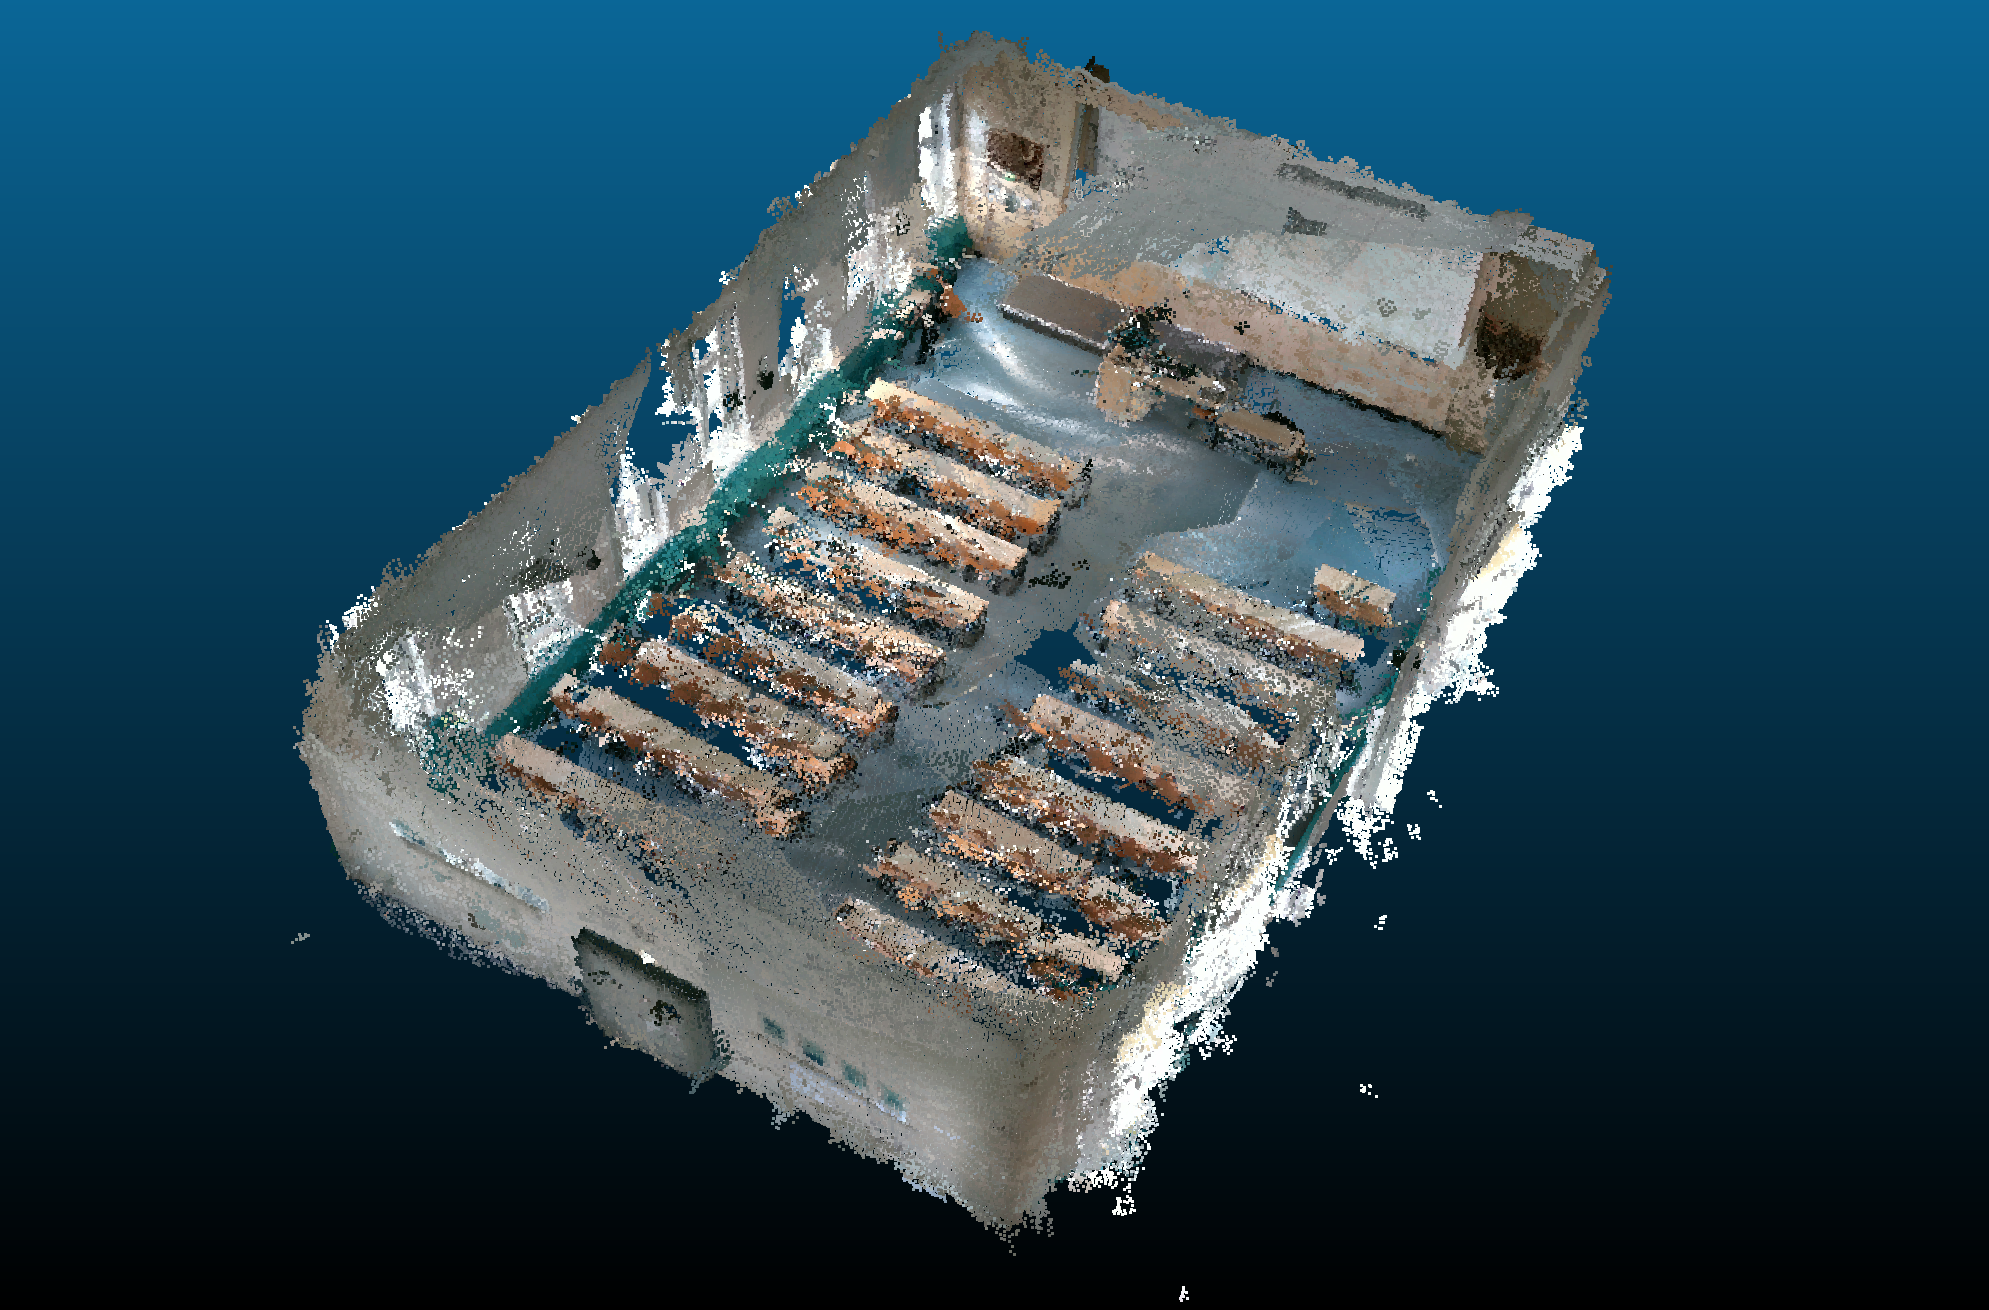
\includegraphics[width=.9\linewidth]{images/307.png}
        \caption[Dynamic Dataset - auditorium]{}
        \label{fig:fin307}
    \end{subfigure}
    \begin{subfigure}{0.5\textwidth}
        \centering
        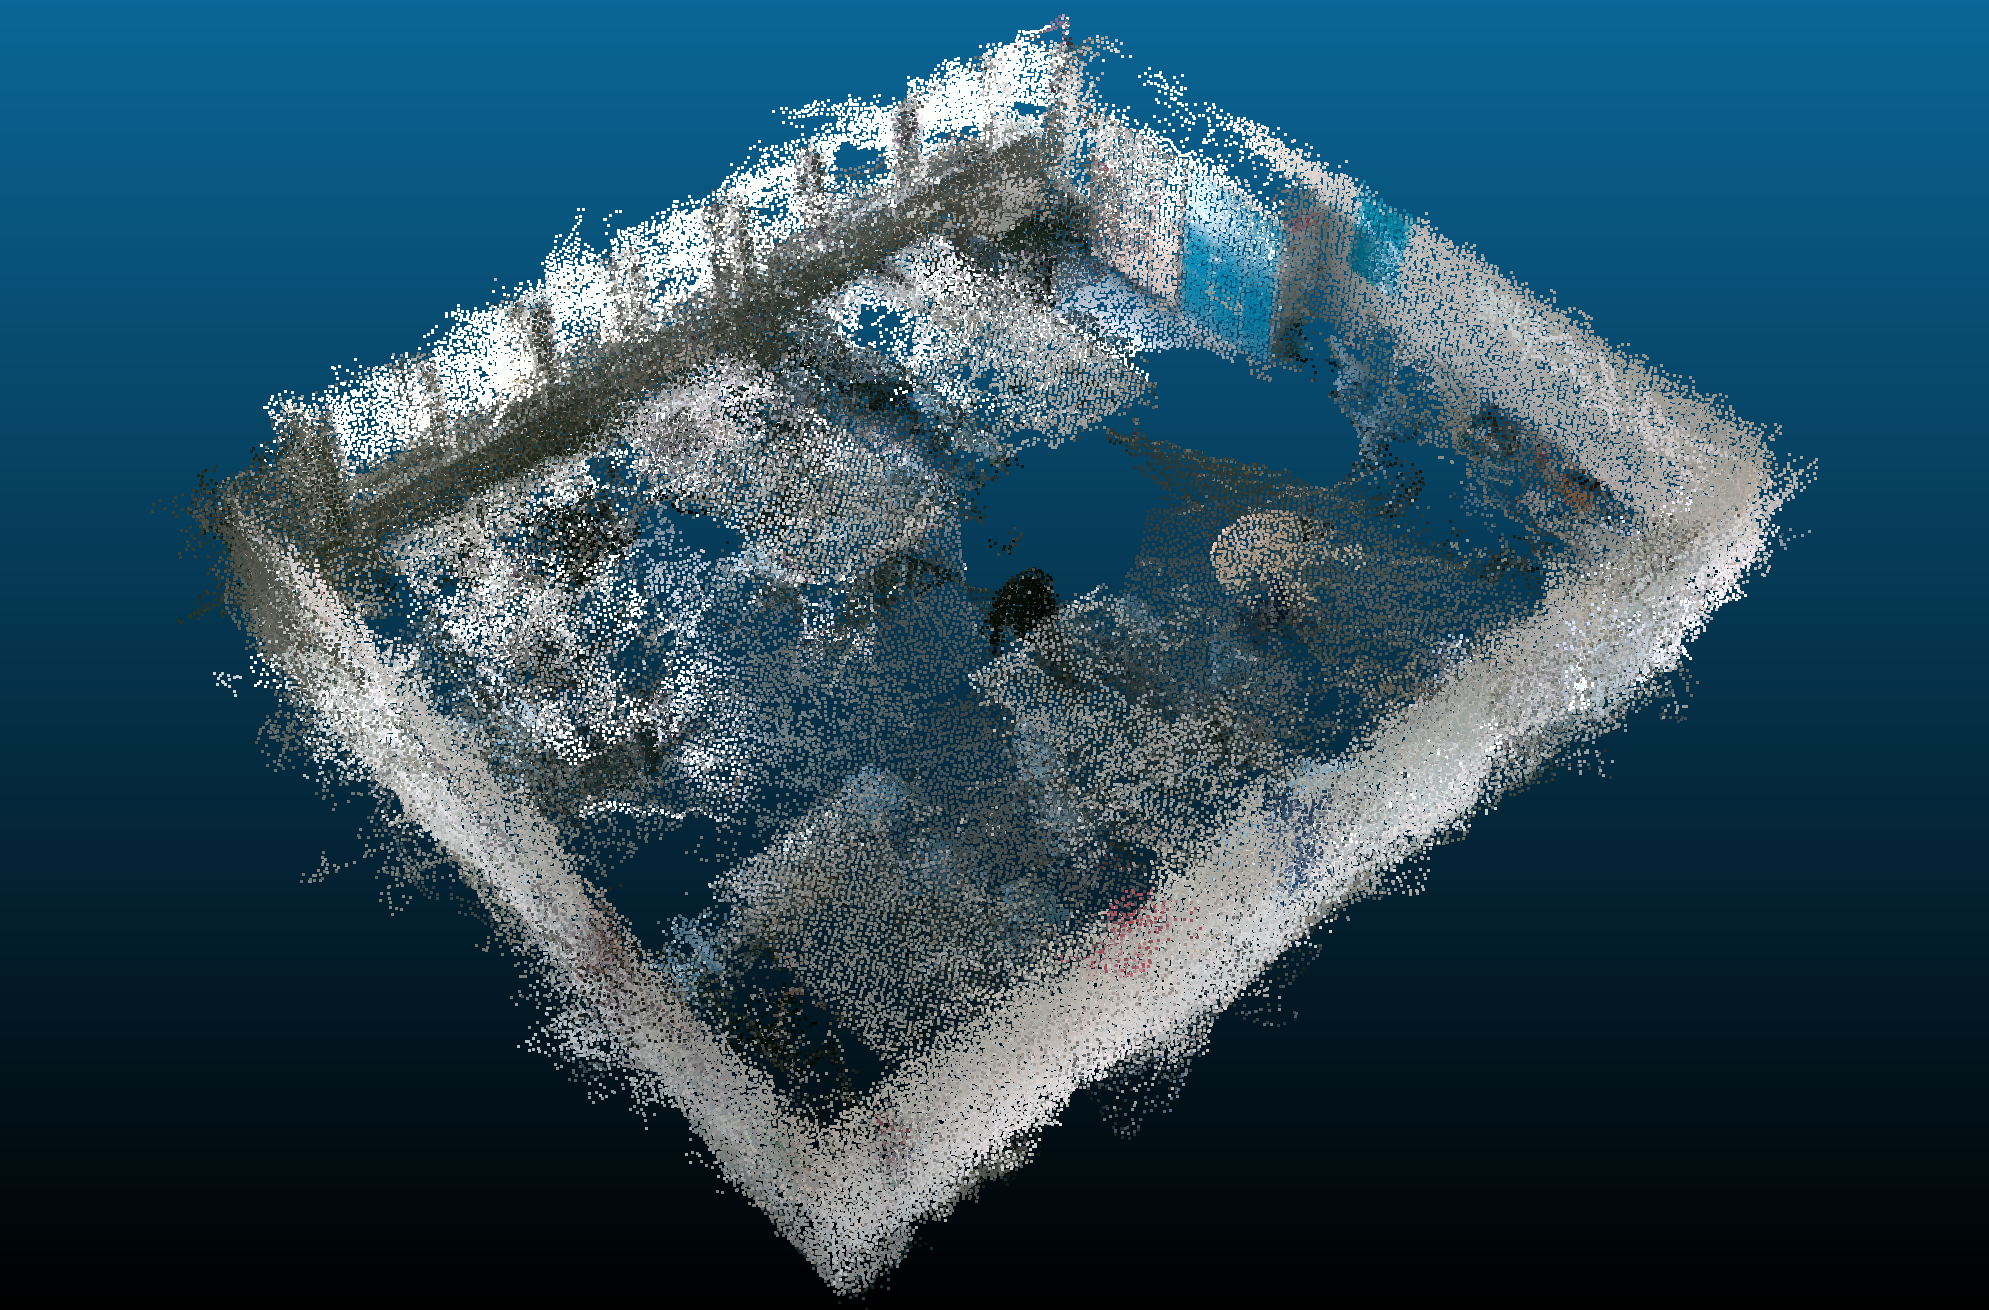
\includegraphics[width=.9\linewidth]{images/333.png}
        \caption[Dynamic Dataset - conference room]{}
        \label{fig:fin333}
    \end{subfigure}
    \begin{subfigure}{0.5\textwidth}
        \centering
        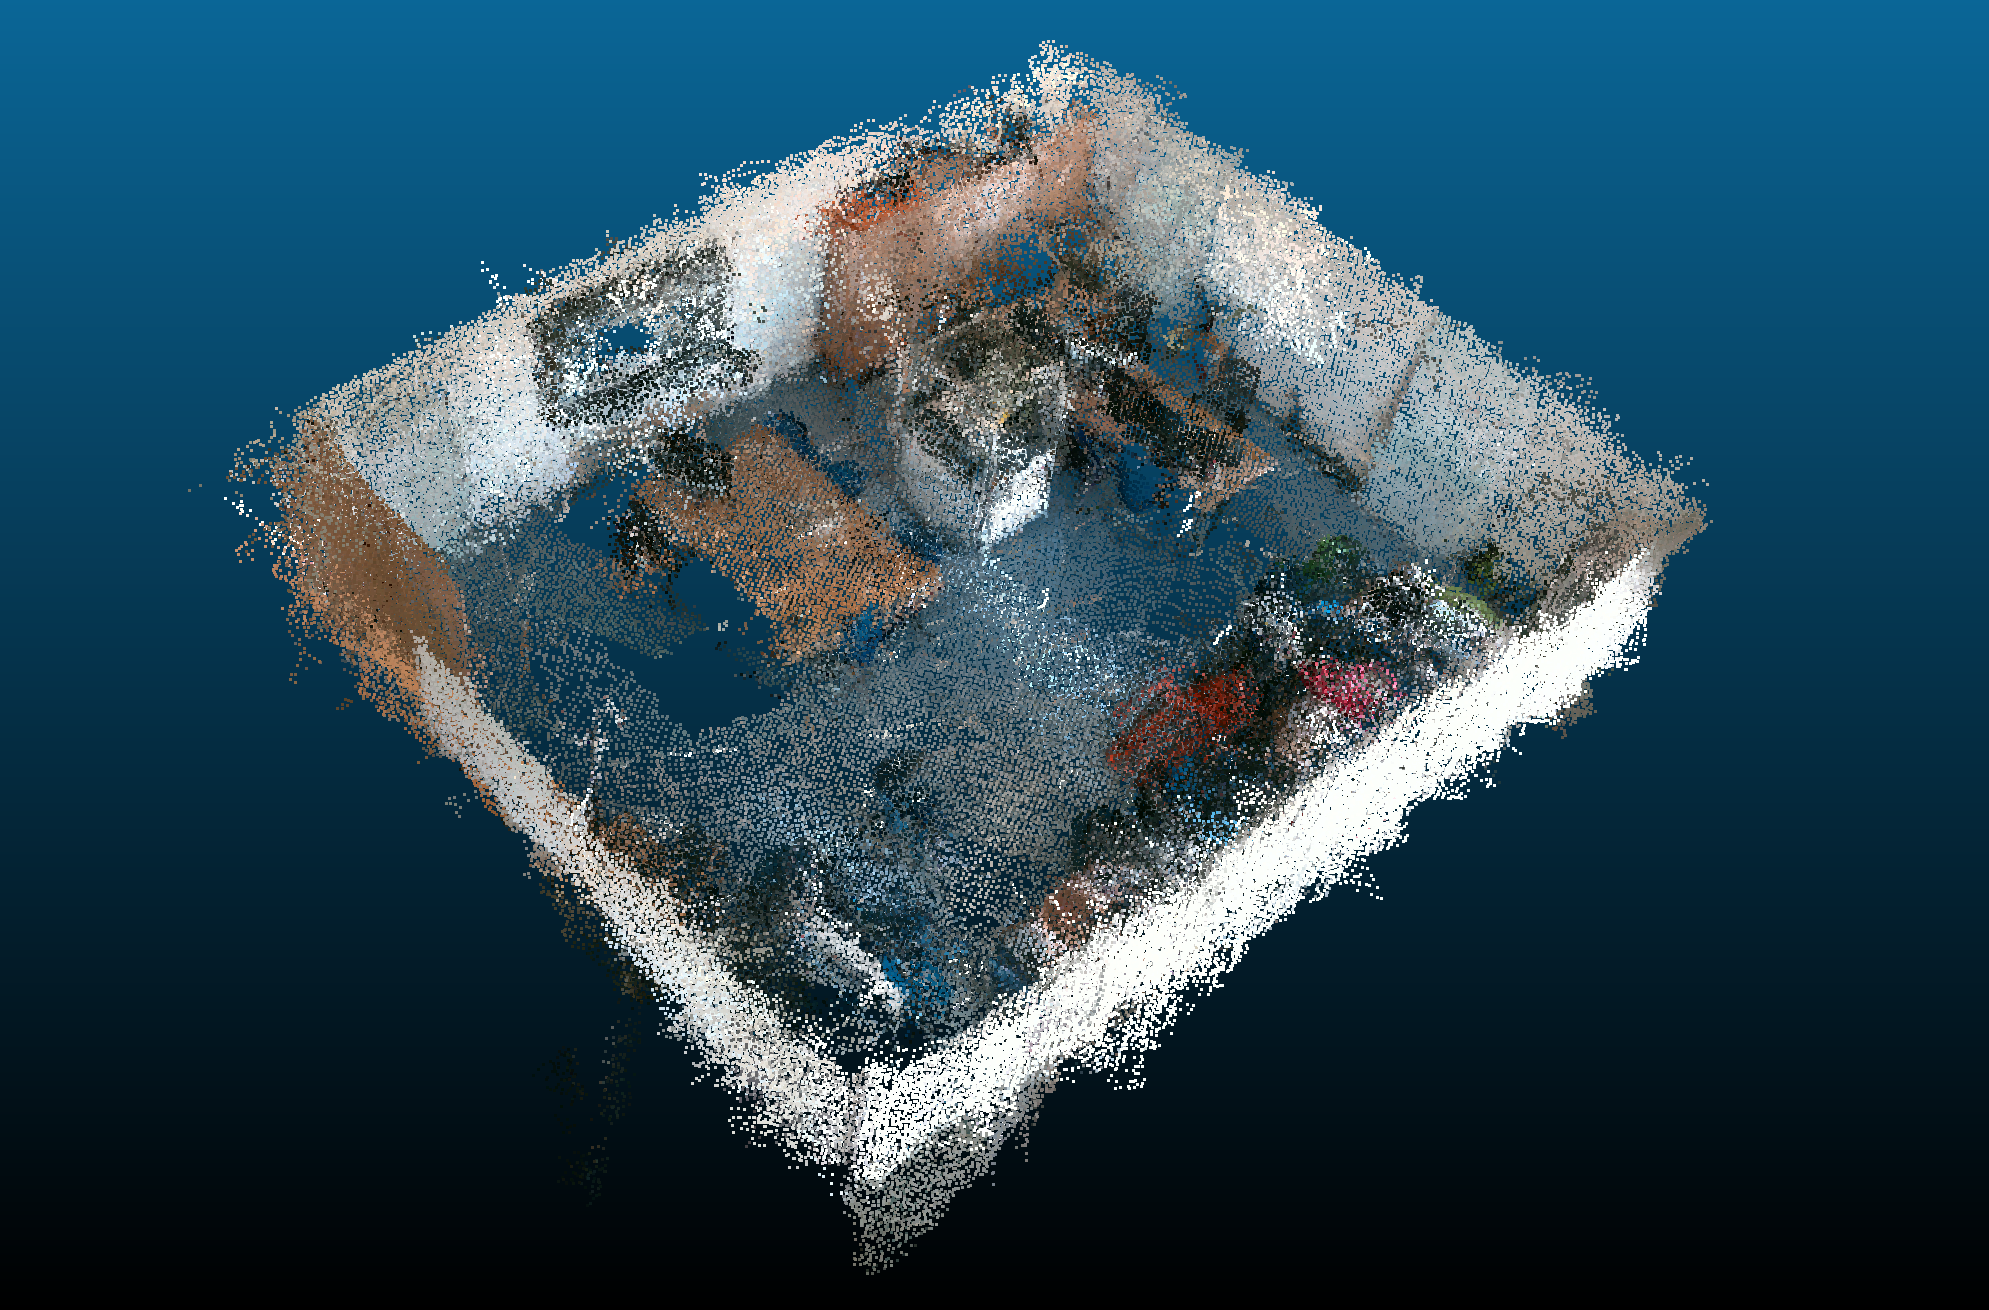
\includegraphics[width=0.9\linewidth]{images/425.png}
        \caption[Dynamic Dataset office]{}
        \label{fig:fin425}
    \end{subfigure}
    \begin{subfigure}{0.5\textwidth}
        \centering
        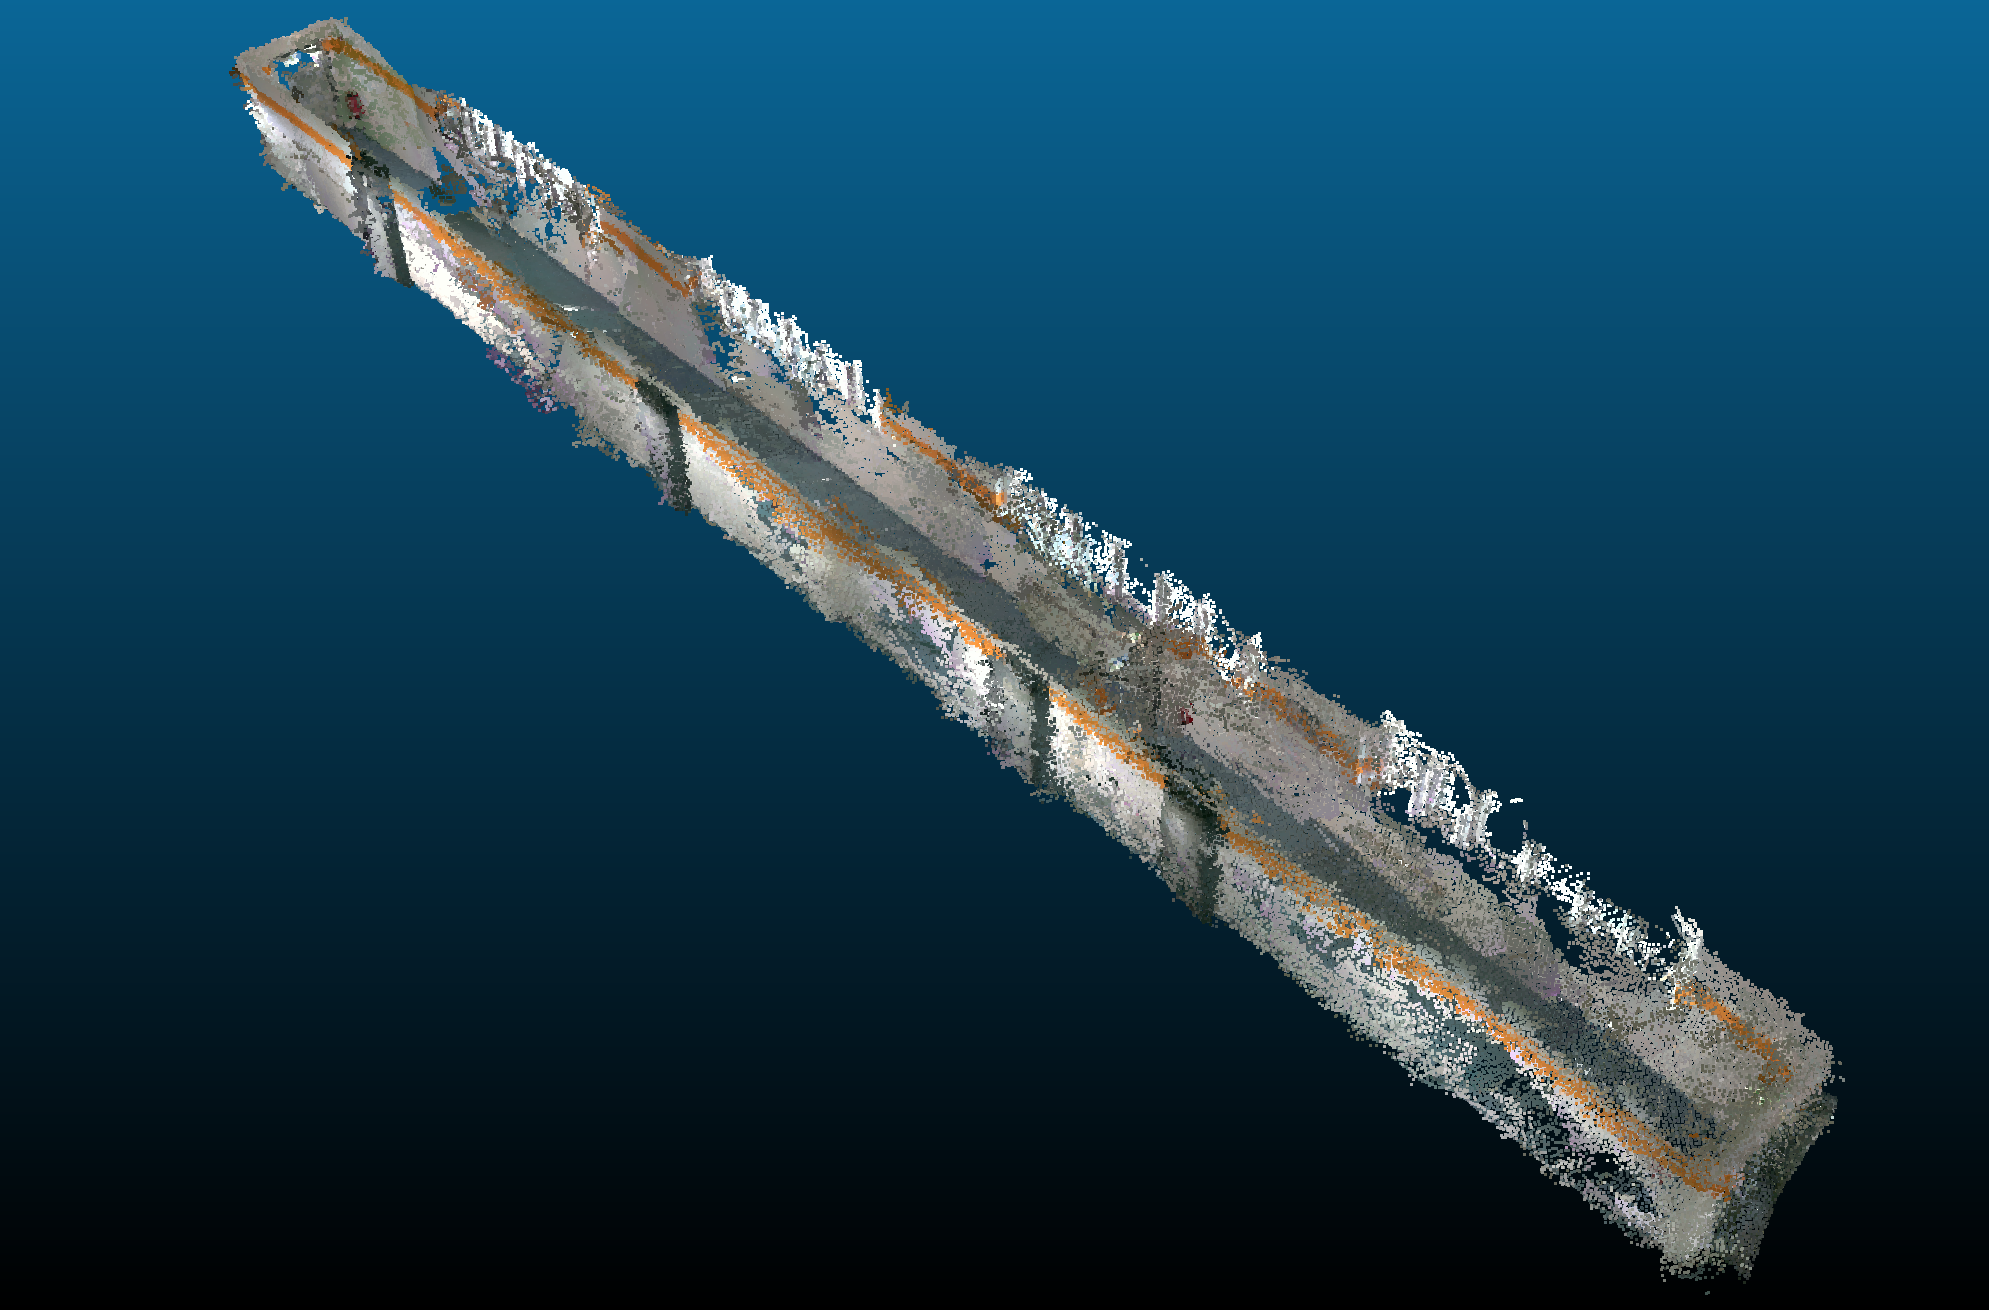
\includegraphics[width=0.9\linewidth]{images/hallway.png}
        \caption[Dynamic Dataset office]{}
        \label{fig:finhw}
    \end{subfigure}
    \caption[Dynamic Datasets]{The recordings for each scene type: (a) auditorium, (b) conference room, (c) office and (d) hallway.}
    \label{fig:fin}
\end{figure}
Lastly, since this is a novel dataset and thus has no ground truth, we create a ground truth. The details thereof are explained in Section~\ref{sec:finimpl}.

% Running \textit{realsense-ros} and holding our cameras, we walk through the aforementioned parts of the building while scanning to the best of our ability.
% We save each incremental map update to a file for later usage.

% Since no ground truth exists for a novel dataset like this, we create a set of ground truth planes $gt_{end}$ for only the most recent update of each scene, e.g., for the entire recording.
% To prepare for the evaluation of a map $m_t$ at a given time $t$, we crop all planes in $gt_{end}$ by removing all points that are not present in $m_t$, as shown in
% Figure~\ref{fig:dynGT}.
% We speed up this expensive process by employing a KD-Tree neighbor search with a small search radius since we only need to know whether a certain point is present or not.
% % Furthermore, we remove planes from the ground truth if the number of included points falls short of a threshold. 
% \begin{figure}[H]
%     \centering
%     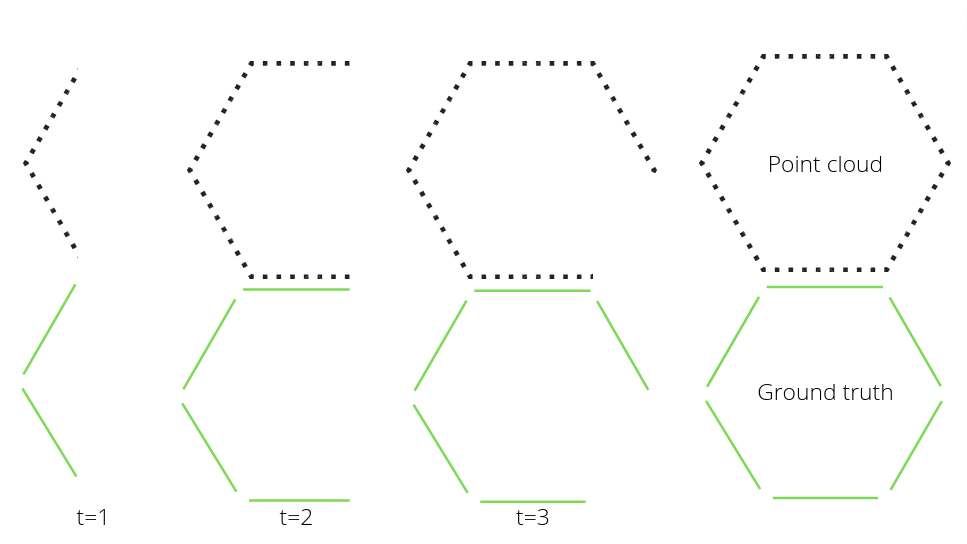
\includegraphics[width=15 cm]{images/dynamic_eval.png}
%     \caption[Dynamic Ground Truth Generation]{Dynamic ground truth generation. All planes that are included in \textit{Ground Truth} are cropped depending on
%         the available point cloud at each time \textit{t} }
%     \label{fig:dynGT}
% \end{figure}


\section{Definition Real-Time}\label{sec:realtime}
% FIXME "wirkt etwas komisch hier. bin mir noch unsicher." 
Finally, to determine whether or not an algorithm runs in real-time, we must first define the meaning of real-time.

We have to consider possible hardware limitations, data flow, and how often it is needed to perform calculations, e.g., how quickly the SLAM algorithm
updates the map (Figure~\ref{fig:concept}, [2]) or how frequent new planes are needed (Figure~\ref{fig:concept}, [4]).

The recorded raw data is not directly sent to the plane detection algorithm but instead given to RTAB-MAP, which then performs
calculations to update and publish the map.
Therefore, the upper limit is the frequency of how often RTAB-MAP publishes those updates, which by default is once per second.
According to this upper limit, we consider an algorithm \textit{real-time applicable}, if it achieves an average frame
rate of minimum 1, e.g., the algorithm manages to process the entire point cloud and detect all planes within one second.

%TODO  Eig nur needed wenn die algos langsamer sind als 1s ODER sollte die cloud extrem wachsen kann man sich auf die 6 meter beschränken, erstmal aber nicht}\\
% \subsection*{reduktion (opt)}
% We can reduce complexity further by taking the specifications (background)
% of the D455 into account. The RMS error of the D455 is reported to be 2\% at 4 meters distance to the sensor.
% Furthermore, the ideal distance is stated to range between $0.6 - 6$ meters.
% To maintain a dense and precise representation of our environment, we therefore limit the detection of planes to a
% radius of 6 meters from the current position.

\section{Summary}
Many applications have constraints in the form of a temporal component. Augmented or Virtual Reality applications that include plane detection
are no exception. In addition to time constraints, good quality is usually tightly coupled to expensive sensors.
% FIXME sprung zu groß
To evaluate to what extent it is possible to perform precise plane detection with a real-time constraint on off-the-shelf hardware,
we compare selected algorithms on the 2D-3D-S and a self-recorded dataset.

\end{document}